% !TEX root = ../../../main.tex
% 来源：中学数学实验教材·第三册（高中数学）
% 章节：不等式和解不等式 / 解不等式
% 原始文件：3.tex，行 1598-1611
% 类型：tikz
% ---
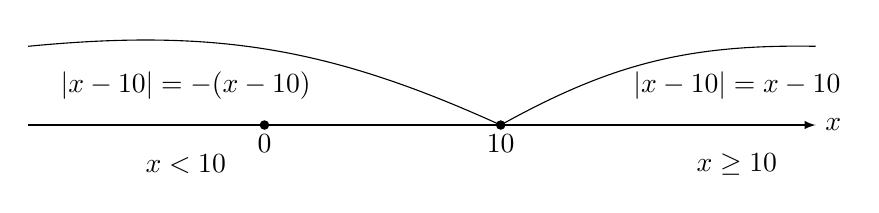
\begin{tikzpicture}[>=latex]
\draw[->](0,0)--(10,0)node [right]{$x$};
\foreach \x/\xtext in {3/0,6/10}
{
    \draw (\x, 0) [fill=black] circle (1.5pt)node[below]{$\xtext$}; 
}    
\draw (0,1) to [bend left=15] (6,0);
\draw (10,1) to [bend left=-15] (6,0);
\node at (2,.5){$|x-10|=-(x-10)$};
\node at (9,.5){$|x-10|=x-10$};
\node at (2,-.5){$x<10$};
\node at (9,-.5){$x\ge 10$};

\end{tikzpicture}
